\documentclass[a4paper,11pt,oneside]{report}

\usepackage{geometry}
\usepackage[utf8]{inputenc}
\usepackage[english]{babel}
\usepackage[T1]{fontenc}
\usepackage{relsize}
\usepackage{color}
\usepackage{listings}
\usepackage{float}
\usepackage{kpfonts}
\usepackage{verbatimbox}
\usepackage{datetime}

% Pour figures en paysage
\usepackage{wrapfig}
\usepackage{lscape}
\usepackage{rotating}

\definecolor{dkgreen}{rgb}{0,0.6,0}
\definecolor{gray}{rgb}{0.5,0.5,0.5}
\definecolor{mauve}{rgb}{0.58,0,0.82}


% more figures per page
\renewcommand\floatpagefraction{.9}
\renewcommand\topfraction{.9}
\renewcommand\bottomfraction{.9}
\renewcommand\textfraction{.1}   
\setcounter{totalnumber}{50}
\setcounter{topnumber}{50}
\setcounter{bottomnumber}{50}

\usepackage{graphicx}
%% \newcommand{\foofoo}{\hspace{-2.3pt}$\bullet$ \hspace{5pt}}


\lstset{
language=C++,
basicstyle=\footnotesize,
numbers=left,
numberstyle=\footnotesize,
stepnumber=1,
numbersep=5pt,
backgroundcolor=\color{white},
showspaces=false,
showstringspaces=false,
showtabs=false,
frame=single,
tabsize=2,
captionpos=b,
breaklines=true,
breakatwhitespace=false,
escapeinside={\%*}{*)}
}


\lstset{
  literate={ù}{{\`u}}1
           {é}{{\'e}}1
           {è}{{\'e}}1
           {à}{{\`a}}1
}


\geometry{margin=2cm}
\geometry{headheight=15pt}
\usepackage{fancyhdr}
\usepackage[xindy,toc]{glossaries}
\usepackage[numbers]{natbib}
\usepackage{fancyvrb}
\usepackage{float}
\usepackage{algorithm2e}
\usepackage{CJKutf8}
\usepackage{tikz-uml}
\usepackage{caption}
\usepackage[footnote,smaller]{acronym}
\usepackage[perpage]{footmisc}
\usepackage{slashbox}
\usepackage[]{titlesec}
\makeatletter
\def\ttl@mkchap@i#1#2#3#4#5#6#7{%
    \ttl@assign\@tempskipa#3\relax\beforetitleunit
    \vspace{\@tempskipa}
    \global\@afterindenttrue
    \ifcase#5 \global\@afterindentfalse\fi
    \ttl@assign\@tempskipb#4\relax\aftertitleunit
    \ttl@topmode{\@tempskipb}{%
        \ttl@select{#6}{#1}{#2}{#7}}%
    \ttl@finmarks  % Outside the box!
    \@ifundefined{ttlp@#6}{}{\ttlp@write{#6}}}
\makeatother

\makeglossaries

\pagestyle{fancy}

\renewcommand*{\acsfont}[1]{\brand{#1}}
\newcommand{\brand}[1]{\textsc{\textbf{#1}}}

\let\oldpar\paragraph
\renewcommand{\paragraph}[1]{\oldpar{#1}\mbox{}\\}

\DeclareMathOperator{\power}{power}
\DeclareMathOperator{\phase}{phase}
\DeclareMathOperator{\recompute}{recompute}

\rhead{Audio watermarking}

\acrodef{MCLT}{Modulated Complex Lapped Transform}
\acrodef{LSB}{Least Significant Bit}
\acrodef{MSB}{Most Significant Bit}
\acrodef{RLSB}{Resistant LSB}
\acrodef{SSW}{Spread-Spectrum Watermarking}
\acrodef{FFT}{Fast Fourier Transform}
\acrodef{GUI}{Graphical User Interface}


\usepackage{hyperref}
\begin{document}
\selectlanguage{english}
\begin{titlepage}
\vspace*{\stretch{2}} 
  \begin{center}

    \textsc{\Huge Audio Watermarking}\\[1cm]
    
  \end{center}
  
  \vspace*{\stretch{2}}
  \begin{flushbottom}
   \begin{flushleft}
    \underline{Students} : Jean-Michaël \textsc{Celerier}, Abdelhamid \textsc{Cherif}, Augustin \textsc{Chevrier}, Alban \textsc{De Martin}, Quentin \textsc{Midy}, Marc \textsc{Queiros Soares}, Valentin \textsc{Sarthou} - \today \\
   \end{flushleft}
  \end{flushbottom}
\end{titlepage}
\clearpage
\tableofcontents
\listoffigures
\newglossaryentry{watermarking}
{
  name=watermarking,
  description={action of inserting a watermark into some data}
}

\newglossaryentry{nulltest}
{
  name={null-test},
  description={checking if two signals are similar by subtracting one to another which causes phase cancellation}
}

\chapter*{Introduction}
In the fields of digital technologies, it is possible to consider an information as a series of bits which represents a message. Thus, watermarking is the technical solution which consists in hiding a message in a given signal. 

This project will deal with the main algorithms used to watermark data in audio signals.

We will first present the theory behind common algorithms, present the evaluation methods, and then move on to the project and implementation parts : how the project was managed, and how the project was implemented.
Finally, we will show the results of our evaluations.

~

~

We wish to thank Mr. Hanna and Mr. Sargent for the help and advices they provided throughout the project.
\chapter{Watermarking}
\section{Presentation}
\section{Existing work}
\section{Techniques}
\subsection{Least Significant Bit}
The most common way to store audio data is by using 16 bit signed integers : it is the Red Book standard (example : figure \ref{fig:audio}).

The audio is divided in samples and a common sample rate (the one given in the Red Book) is $44\,100$ Hz. The audio is encoded using pulse-code modulation : each sample roughly equates the average voltage measured by the analog-to-digital converter during one $44\,100$th of a second.

\begin{figure}[h!]
\centering
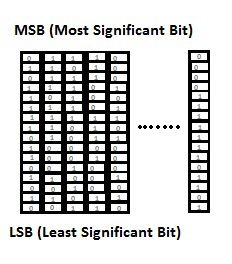
\includegraphics{images/LSB1.jpg}
\caption{Example : some samples of Red Book audio}
\label{fig:audio}
\end{figure}


The principle of the \ac{LSB} method \cite{tirkel1993electronic} is to encode the watermark on the $16$th bit of the samples as visible on figure \ref{fig:lsb}.

\begin{figure}[h!]
\centering
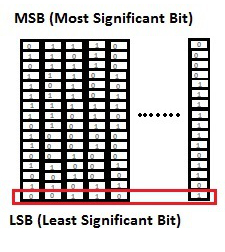
\includegraphics{images/LSB2.jpg}
\caption{LSB watermarking : the watermark is put in the $16$th line of bits, inside the red rectangle}
\label{fig:lsb}
\end{figure}

This method presents two main advantages. 
\subsubsection{Advantage: Quantity of embeddable data}
The quantity of information watermarkable in the signal is quite high : we are able to encode 1 bit per sample. In order to give an order of magnitude, for a music track of a common length of 2 minutes, with a sampling frequency of $44\,100$ Hz, the \ac{LSB} method would allow to encode $5\,292\,000$ bits, which is about 645 kbytes, i.e. about the size of a long text, an image and even short audio signals. 
\subsubsection{Advantage: Simplicity}
The method is really simple to implement.
The algorithm is present on \ref{algo:lsb}.

\begin{algorithm}
\DontPrintSemicolon
\KwIn{A finite set $B=\{b_1, b_2, \ldots, b_m\}$ of data bits to hide}
\KwIn{A finite set $S=\{s_1, s_2, \ldots, s_n\}$ of audio samples}
\KwOut{A finite set $W=\{w_1, w_2, \ldots, w_n\}$ of watermarked audio samples}

\For{$i \gets 1$ \textbf{to} $m$} {

  $w_i \gets s_i$ \;  
  $w_i [16] \gets b_i$ \;

}

\Return{$W$}\;

\caption{\ac{LSB} Watermarking. For the sake of simplicity, the audio samples are considered to be arrays of bits, where $s[1]$ is the \ac{MSB} and $s[16]$ the \ac{LSB}.}

\label{algo:lsb}

\end{algorithm}

\subsubsection{Advantage: Lack of audibility}
The distortion of the signal after encoding the watermark is very weak. Indeed, the least significant bit of a $16$ bits digital signal affects the amplitude of the signal by a value of $\displaystyle\frac{1}{2^{16}} * V_{cc}$\cite{kester2005data}, with $V_{cc}$ the maximum voltage that the sound card is able to create.
Finally, the LSB method gives a maximum signal-noise ratio of : 
 
\begin{center}
\begin{math}
10 \log \displaystyle\frac{V_{cc}}{V_{cc} - \displaystyle\frac{1}{2^{16}} * V_{cc}} \simeq 10^{-4}
\end{math}
\end{center}

\subsubsection{Drawback: Easy interception}
Despite these advantages, the LSB method has a main drawback : the watermark is very simple to decode. If someone wants to intercept the hidden signal, he just has to take the $LSB$ of the transmitted signal's samples to know the content of the watermark.  

\subsubsection{Drawback: Fragility}
Another important point is that this does not resist well to audio distorsions, and compression (the 16th bit is generally very close to the noise floor, hence a lossy compression like MP3 will damage the watermark and make it unreadable). 

\subsubsection{Other approaches to LSB method}
In this project, two further approaches of the \ac{LSB} are proposed :
\begin{itemize}
\item Rather than only encoding the watermark on just one line of bits, it could be encoded on several lines of bits. For example, the three last bits of each samples would serve to encode the watermark. The encodable quantity of information hence increases three-fold. We implemented this capability in our \ac{LSB} algorithm.
\item In order to increase the resistance to the attacks and to the noise, it could be interesting to encode the same watermark on several lines of bits. For example, the same watermark bit would be encoded on the three last bits of each sample. We implemented this method in our software and named it \ac{RLSB}.
\end{itemize} 

These two methods increase either redundancy or capacity at the cost of an increased noise floor.

To conclude, the \ac{LSB} method is inaudible and it provides a huge watermarking rate in comparison to the other methods. However, the watermark encoded by this algorithm is not really hidden and it does not resist to lossy compression and audio attacks.

We choose to use this algorithm as a base to test our software and provide a working example and a lowest common denominator for benchmarks.
\subsection{Spread-spectrum Watermarking}

The purpose of the \ac{SSW} method is to embed the hidden data of the watermark in the frequency domain of the host signal. Hence, \ac{SSW} algorithm relies on a time-to-frequency transform and on its inverse transform. In fact, any frequency transform can be used with this method, as long as the same transform is used for watermarking insertion and detection. For example, in this project, we used the Discrete Fourier Transform.

~

The core of this method is based on a random sequence of N numbers, whose values are either $1$ or $-1$, with a equal distribution for both. This sequence is the key of decryption and thus must be known by the emitter and the receiver.

~

Therefore, the first step is to generate this sequence.

\subsubsection{Watermark insertion}

In order to embed data with the \ac{SSW} method, the host signal must firstly be divided into chunks of given size (for example, chunks of $512$ samples). The \ac{SSW} algorithm can then be applied to each of these chunks in order to embed the hidden data. Only 1 bit of hidden data can be embedded in a chunk.

~

On each chunk, the frequency transform is then applied. The result is an array of half the size of the chunks, each cell of it containing the energy and phase for a certain frequency bin of this chunk.

~

The next step is to select N (the size of the random sequence) frequency bins that are going to be modified. Therefore, N has to be less than half the chunk size. The goal is to avoid inaudible portions of the frequency spectrum because they are more likely to create audible noise when modified. The best is to keep frequency bins in the $200$ Hz - $2$ kHz subband.

~

Let's call $F$ the sequence of the magnitudes (in decibels) of the selected frequency bins and $S$ the random sequence. The following computation is then performed in order to insert 1 bit of hidden information into 1 chunk:

~

$F[i] = F[i] + W[k] \times \delta \times S[i]$, for $i$ varying from 1 to N.

~

\noindent where $W$ is the hidden data to be embedded ($W[k]$ is equal to 1 for bit 1 and -1 for bit 0), $k$ the current bit of hidden data and $\delta$ the amplitude of the watermark (usually between $0.5$ and $2.5$ dB).

~

After the modification on the frequency magnitudes, the time signal is reconstructed using the original phases and the inverse frequency transform.

\subsubsection{Watermark detection}

Just like in the embedding part, the signal must be divided into chunks. They have to be the same size as during embedding.

~

The frequency transform is also applied and the same frequency bins as before are also selected. Magnitudes in decibels are computed as well but instead of modifying them, a correlation is calculated, just as follows :

~

$C = F \cdot \delta S$

~

\noindent where $F$ is the sequence of selected frequencies magnitudes, $S$ the random sequence and $\cdot$ the normalized dot product.

~

When the chunk has not been watermarked, $C$ should be close to $0$ because $F$ would be close to a random sequence, and when the chunk is watermarked, $C$ should be closer to $1$ because $F$ would be equal to $random + \delta S$ and $\delta S \cdot \delta S = 1$. When the bit 0 is embedded, $F$ is equal to $random - \delta S$, so $C$ should be closer to $-1$.

~

Hence, for each chunk, it is possible to determine whether or not there is a watermark (by using a threshold) and if so, which bit of data is embedded. Doing it for each chunk allows for the reconstruction of the entire hidden data.

~

A bigger $N$ would allow better correlation values but also a more audible watermark. The same rule applies to $\delta$.

~

There are several methods that can improve watermark detection, like cepstrum filtering, but these were not implemented in this project.

\subsection{Compression-Expansion}\cite{foo2010}

Compression-expansion is a time-based method for watermarking, unlike S.S.W. which is a spectral-based method.\\
Its purpose is based on dividing a signal into segments of frames that overlap each other, calculate a local mask and taking specific coefficients according to the mask previously calculated from a frame to add them to the end of the following one. The technique is detailed in this subsection.

\paragraph{Purpose of the compression-expansion of segments}
Let's consider a signal. One divide it into segments that are containing the same number of frames.\\
The division must be in respect of the following purpose : each segment half-overlaps the following one. A Hanning window is then applied to the segments, as showed by the following figure :
\begin{figure}[H]
\center{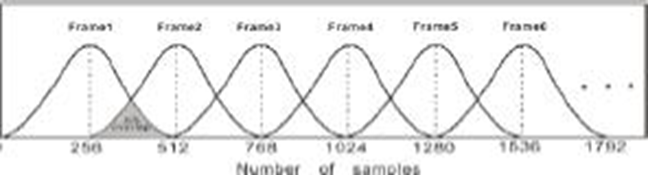
\includegraphics{images/Image1.png}}
\caption{\label{frames} Division into frames of a signal}
\end{figure}
For each bit of the watermark, two segments are used. So that no confusion is made, the third segment that follows the two segments used is left.\\
A discret cosine transform (D.C.T.) is applied on the two segments that are under consideration. Here is used a local auditory mask, which is calculated thanks to a psychoacoustic model. We will see later how this mask is calculated.

According to the mask, in the first segment, one takes the 8 first coefficients of the D.C.T. that are greater than the mask. One must look for those coefficients from the end of the segment. As one has removed coefficients from a segment, it is compressed\\
Those coefficients are then added to the beginning of the following segment. It is thus expanded.\\
The following figure sums up this operation :
\begin{figure}[H]
\center{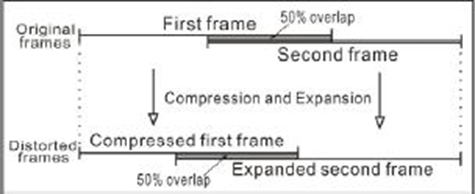
\includegraphics{images/Image2.png}}
\caption{\label{compression-expansion} Compression and expansion of the segments}
\end{figure}

An inverse D.C.T. is applied then to come back to the time domain. The differences between the original signal and the reconstructed one yields a signal made up of little waveforms that have the shape of a diamond, such as this figure shows :
\begin{figure}[H]
\center{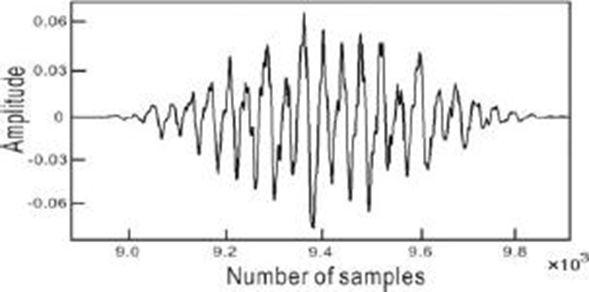
\includegraphics{images/Image3.png}}
\caption{\label{diamond} Diamond obtained by the difference of original and reconstructed waveforms}
\end{figure}

\paragraph{Use of the diamonds}
Depending on the original signal, either mono, either stereo, the method differs. In each case, the diamonds that are previously obtained by the difference of the original signal and the reconstructed one are used, but in different ways.

Let's consider a mono signal. The principle is here to obtain a diamond to embed the bit "1" (therefore, apply the method described in the previous paragraph), and nothing to embed the bit "0" (no calculation).\\
As it is not sure that the processing of this type of watermarking begins exactly at the beginning of the signal, one must know where's the first bit embedded. One considers then that, when the encoding begins, a diamond is calculated.

For a stereo signal, one uses the two channels. On the left channel, a diamond is calculated to embed "1", and the other way round for "0" (on the right channel). The two channels enables the fact that there can be blanks on both channels at the same time, therefore having different time intervals between the diamonds.
\begin{figure}[H]
\center{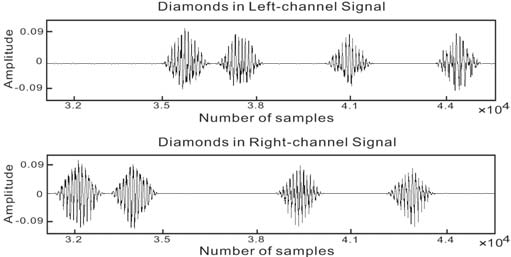
\includegraphics{images/Image5.png}}
\caption{\label{stereo watermarking} Series of diamonds for a stereo signal}
\end{figure}

The next step is to detect those diamonds. The main problem generated by the compression-expansion is that, in some cases, the distortion can be difficult to detect (the diamonds are to tiny), as this is showed in this figure :
\begin{figure}[H]
\center{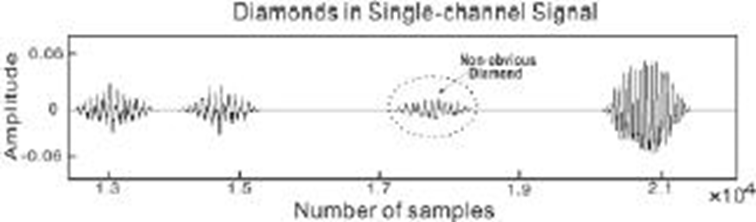
\includegraphics{images/Image4.png}}
\caption{\label{distortion} Example of a to much tiny diamond}
\end{figure}

Such a problem can be easily avoided in stereo signals, because the watermarks can be separated with blanks on both channels. But on a mono signal, if the diamond is considered as noise (therefore, not taken into consideration), it will yield a false detection of the watermark. This is a constraint for mono signals : some types of signals (such as those which encode speeches) can't be used to ensure a good accuracy. These types of signals have often parts where the energy is low, which means a low amplitude. As the diamond is obtained by taking the difference of the original signal and the reconstructed one, this difference is as low as the amplitude of the signal is weak.

To detect the watermark inside a signal, the original non-watermarked signal is needed to calculate the diamonds. The detection of the diamonds can be done with several methods : some are described here.\\
\begin{itemize}
\item \textbf{Sum of absolute difference} : one computes the sums of absolute differences between the watermarked signals and the original signals. So as to detect a diamond, which duration is equal to 2 segments of frames that overlap each other by 50\% in the signal, in addition to one frame unused due to the 50\% overlap, each sum is calculated on the base of 3 segments as described previously. On the one hand, when there is a diamond (thus, a distortion on the watermarked signal), the sum of the absolute values of the differences during the distortion is found to be greater than 5,5. On the other hand, the sum of the absolute values of the differences is always under 0,8. Thus, a threshold of $\frac{5,5 + 0,8}{2} = 3,15$ can be taken to detect a diamond.\\
This method is very simple and very accurate when no attack is done on the watermarked signal. But when it is damaged, several errors of detection can be made.
\item \textbf{Calculation of gradients} : a diamond has two slopes that make the shape of a triangle, such as showed on the figure below :
\begin{figure}[H]
\center{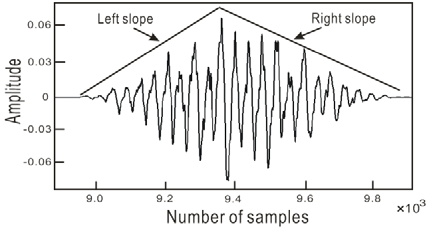
\includegraphics[scale=0.7]{images/Image6.png}}
\caption{\label{slopes} The slopes for a diamond}
\end{figure}
The derivative of each slope should be a constant non-zero function. It is experimentally found that the constant values of these function are greater than 1.7 for the left slope and lower than -1.5 for the right slope. These criteria can be used to ensure that the segments considered where used to calculate a diamond or not.\\
From the experience, this type of searching works well on attacked signals with noise and re-sampling. Nevertheless, the results are less satisfying when the watermarked signal is compressed using a low-pass filter or M.P. 3 algorithm.
\item \textbf{Cross-correlation with reference triangle} : Experimental results show that the amplitudes of the diamonds using different types of audio signals are quite similar. Therefore, for a segment of 512 samples, the length of the envelope is the same as the one of the diamond, which is 768 samples ($\frac{3}{2}$ times the segment length). The average amplitude is 0,06 in the middle of the envelope (if the frame size changes, then these values are no more applicable).
\begin{figure}[H]
\center{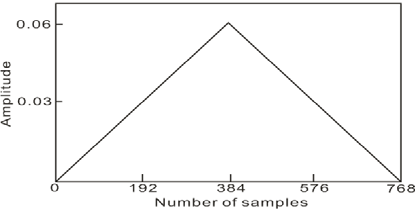
\includegraphics[scale=0.7]{images/Image7.png}}
\caption{\label{envelope} Envelope for a watermark extraction}
\end{figure}
The cross-correlation between this shape and the signal with the diamonds is calculated. If the value is near 1, it means there is a diamond, whereas if it is near 0, there are non-distorted frames.\\
Experiments indicate that a cross-correlation value over 0,78 is a diamond and under 0,31 represents non-distorted frames. If the value is between 0,78 and 0,31, then another detection method is applied. This method gives higher detection accuracy than the previous one.
\end{itemize}

\paragraph{Calculation of the mask}
The signal is segmented into overlapped frames. Then, the short time Fourier transform is applied in order to get a spectral representation. However, another scale is used : the Bark Scale. The concept of the Bark scale is based on a psychoacoustic phenomenon : the basilar membrane in the hearing mechanism analyses the incoming sound through a spatial-spectral analysis. This is done in small regions of the basilar membrane called “critical bands”.\\
The \textbf{Bark scale} is obtained from the frequency range with the following formula :
$$z_i = 13\textnormal{tan}^{-1}\frac{0,76f_i}{1000}+3,5\textnormal{tan}^{-1}\left(\frac{f_i}{7500}\right)^2$$
In the following graph is given the spectral representation of the 7\textsuperscript{th} segment of the file \textbf{\textit{input\_mono.wav}}, given in the folder \textbf{\textit{output}}. This was calculated with \textbf{\textit{MatLab}} :
\begin{figure}[H]
\center{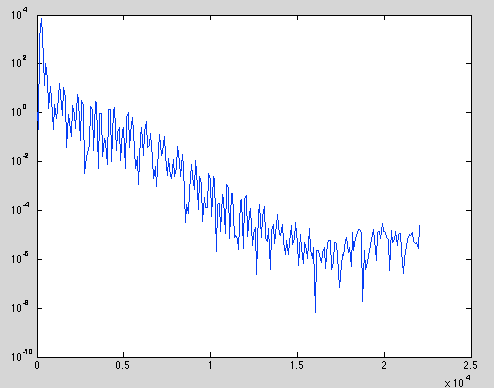
\includegraphics[scale=0.5]{images/Image8.png}}
\caption{Spectral representation of the 7\textsuperscript{th} segment of \textbf{\textit{input\_mono.wav}}}
\end{figure}

Then, one needs to calculate the power spectra. The formula is given below :
$$S_p(j\omega) = 	|\mathcal{F}(s(t)w(t))|$$
where $sw(t) = s(t)w(t)$ is the windowed segment, and $\mathcal{F}$ is the Fourier transform (which explains the transformation from $t$ to $j\omega$).

For each critical band of the basilar membrane, one computes its energy as follows :
$$S_{pz}(z) = \sum_{\omega = LBZ}^{\omega = HBZ}S_p(j\omega)$$
where $LBZ$ and $HBZ$ are respectively the lower and higher frequencies of the critical band. z goes from 1 to the total of critical bands, and one does the sum to get the total energy.\\
In the graph below is represented in red the energy per critical band :
\begin{figure}[H]
\center{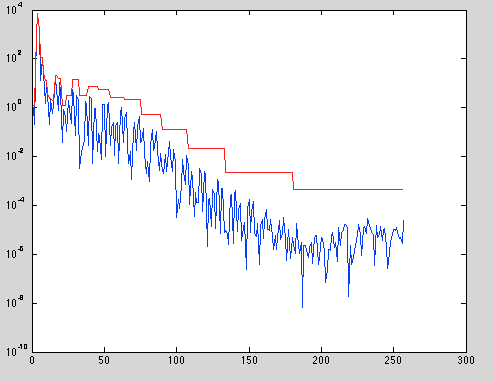
\includegraphics[scale=0.5]{images/Image9.png}}
\caption{Energy per critical band and spectral representation}
\end{figure}

At this step, one needs also to compute the basilar membrane spreading function. This function determines how much of the energy of each 
critical band is contributed to the neighbouring bands.\\
This function in dB is :
$$B_k = 15,91+7,5(k + 0,474) - 17,5\sqrt{1 + (k + 0,474)^2}$$
k takes its values in $\mathbb{Z}$.
\begin{figure}[H]
\center{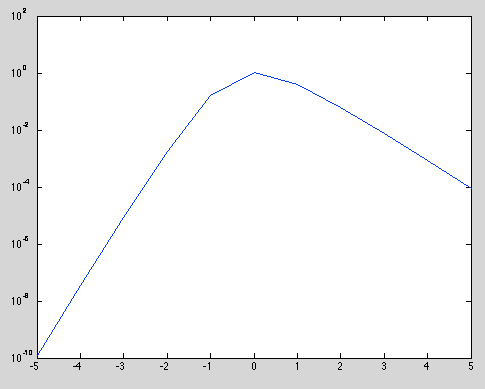
\includegraphics[scale=0.5]{images/Image10.png}}
\caption{Representation of $B$ in function of $z$}
\end{figure}
The spreading across bands is computed by the convolution of the previous function and the energy per critical band :
$$S_m(z) = S_pz(z)*B(z)$$
\begin{figure}[H]
\center{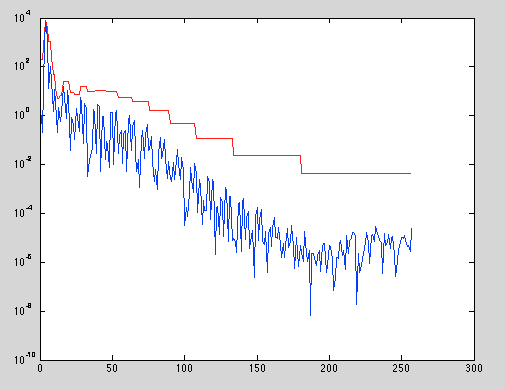
\includegraphics[scale=0.5]{images/Image11.png}}
\caption{Representation of $S_m$ as a function of z (red curve)}
\end{figure}

With the different things computed, one can now calculate the masking threshold.\\
First, one must get the spectral flatness measure :
$$SFM = 10\textnormal{log}\left(\frac{\prod_{z = 1}^{z = Z_t} S_{pz}(z)}{\frac{1}{Z_t}\sum_{z = 1}^{z = Z_t} S_{pz}(z)}\right)^\frac{1}{Z_t}$$

One can now have the tonality factor $\alpha$ :
$$\alpha = \textnormal{min}\left(\frac{SFM}{-60} ; 1\right)$$

The masking threshold is given by :
$$T_{norm}(z) = \frac{10^{\textnormal{log} S_m(z)-\frac{O(z)}{10}}}{P_z}$$
where $O(z)$ is the masking energy offset :
$$O(z) = \alpha(14,5 + z) + 5,5(1 - \alpha)$$
and $P_z$ is the number of points in each band $z$, $z \in [\![1 ; Z_t]\!]$.

\paragraph{Results of the method}
Experiments have been made on three types of signals :
\begin{itemize}
\item rock music
\item classical music
\item male speech
\end{itemize}
Rock music have a very high signal energy, unlike classical music. A speech has also a moderate signal energy, but sequences are very energied-low.\\
All signals are sampled at 44,1 kHz and quantized with 16 b. Files are either mono (segment size : 512), either stereo (segment sizes : 256, 512 or 1024).

The information was a binary $64\times64$ image.

The audio quality of the watermarked signal was measured with several methods. Listeners evaluated the quality through comparing both original and modified signals. And to get more objective results, the signal to noise ratio (S.N.R.) was used. This is given by the formula :
$$SNR = 10\textnormal{log}\frac{\sum_{n} x(n)^2}{\sum_{n} (x(n) - y(n))^2}$$
where $x$ is the original signal and $y$ the watermarked one.\\
This experiment leads to conclude that the watermarked signals are not damaged perceptually. Furthermore, the S.N.R. values obtained for watermarked signals are around 40 dB. Notice that, for stereo signals, the S.N.R. is calculated on each channel.\\
The requirement of the I.F.P.I. (International Federation of the Phonographic Industry) is 20 dB. Therefore, it can be concluded that the watermarks do not affect the signal perceptually speaking.

To test the robustness, several attacks were made. The robustness is calculated with the bit error rate, which is the number of false bits recovered divided by the total number of bits.\\
The attacks were :
\begin{itemize}
\item Attack free
\item Noise addition (decrease of the S.N.R. of 20 dB)
\item Re-sampling (down-sampling to 22,05 kHz and up-sampling to 44,1 kHz then)
\item Re-quantization (down-quantized to 8 b and up-quantized to 16 b again)
\item Echo adding (delay : 0,001 s)
\item Low-pass filtering (cutoff frequency at 6 kHz)
\item M.P. 3 compression (32 kb/s)
\item Amplitude variation (increased of 30 \% and decreased then by 20 \%)
\item Time-scale modification (lengthened by 10 \% and decreased then by 5 \%)
\item Pitch scaling
\end{itemize}

From the results obtained, stereo signals are better to enclose a watermark. Mono signals are easier to be attacked, and the information recovered is false. The same observation is made when the segments have too low frames. It is because the maximum amplitude of the diamonds are lower as the segments are smaller.\\
Compressions, which are generally damaging, are here well supported.

\chapter{Evaluation}
\section{Main evaluation idea}
\section{Existing work}
\section{Evaluation methods}
\chapter{Organization and project management}
In this chapter, we will study how the project was managed, and the different steps we had to take in order to achieve all our goals.

\section{Technologies and methods}
We saw this project as a way to enact modern software development techniques.
\subsection{Agile methodology}
Even if we didn't explicitely named it, the method used was clearly agile, because every week or every two weeks we saw our clients and showed them our current progress, and we stated the goals for the following weeks.

\subsection{Softwares used}
We also used different software tools to manage the project.

\paragraph{Git and Github} 
They were used to hold the source files and the wiki. We also put our weekly reports here, which allowed the teachers to tell us what we had to improve. \brand{Git} is very useful for advanced softwares, even if we didn't use it to its maximum potential.
As well, we did not use every single feature of \brand{Github}, like bug reports.

\paragraph{Travis CI} 
A big advantage of Github is that it allows continuous integration with other services. We used \brand{Travis CI}. The idea is simple : everytime somebody does a commit, a remote build system fetches it, and tries to build it and runs an user-specified script (in our case, unit tests). If the build fails, or if the software ends in an erroneous state like with a segmentation fault, we get an email, and we can access the build and execution log to see what failed.

This can be used as a testimony to check that the project correctly builds on a minimal system.

\paragraph{Doxygen} was used for the documentation. Mostly everything is documented, the library as well as the graphical interface.

\paragraph{QtCreator} was the chosen development environment. It has a tight integration with \brand{qmake} as a build system, hence the hard dependency on it (which is anyway included with \brand{Qt}, required for the user interface). 

\paragraph{Qt Test Framework}
This test frameworkwas used for the unit testing, in order to provide an easy-to-read output. It can also provide an Xunit XML output which is a standard unit test output, but we did not feel the need for it. 

\paragraph{cppcheck}
It is a static code analysis software which finds bugs unlikely to be found by a compiler, like memory leaks, array bounds overflow... We ran it regularly to check for potential bugs.

\paragraph{valgrind}
A big emphasis was put on the memory cleanliness : as a matter of fact, there is not a single memory leak in the library, thanks to the extensive use of smart pointers (there is not a single free pointer in our classes, they are all embedded in \texttt{std::smart\_ptr} objects).

We only noted a bug with the \ac{MCLT} that we did not had the time to solve, however it is not used in the main software so it is not really relevant.

\paragraph{lcov}
This software was used to test the code coverage of the library during the unit tests, to ensure maximum efficiency for the other tools that we explained before.

The output is present in the folder \texttt{html-coverage}. The tests cover almost $90\%$ of the code (we could not do more because of lack of time).

\section{Schedule}
We will see here the repartition of the work on the project.

An important thing to keep in mind is that the project used an existing framework, which had some bugs : this helped to alleviate much of the required work.

\subsection{Work repartition}
The repartition was as follows : 
\begin{figure}[h!]
\centering
\begin{tabular}{|c|l|}
\hline
Person & Work done \\
\hline
Jean-Michaël Celerier & Work on the framework, project management \\
Abdelhamid Cherif & Evaluation \\
Augustin Chevrier & Compression-expansion method \\
Alban De Martin & \ac{GUI} \\
Quentin Midy & \ac{LSB} Methods \\
Valentin Sarthou & \ac{SSW} Methods \\
Marc Queiros Soares & Compression-expansion method \\
\hline
\end{tabular}
\end{figure}

\subsection{Gantt Diagram}
A Gantt diagram was made to have an assessment and a track to follow. It is viewable on the next page.

\begin{sidewaysfigure}[h!]
\centering
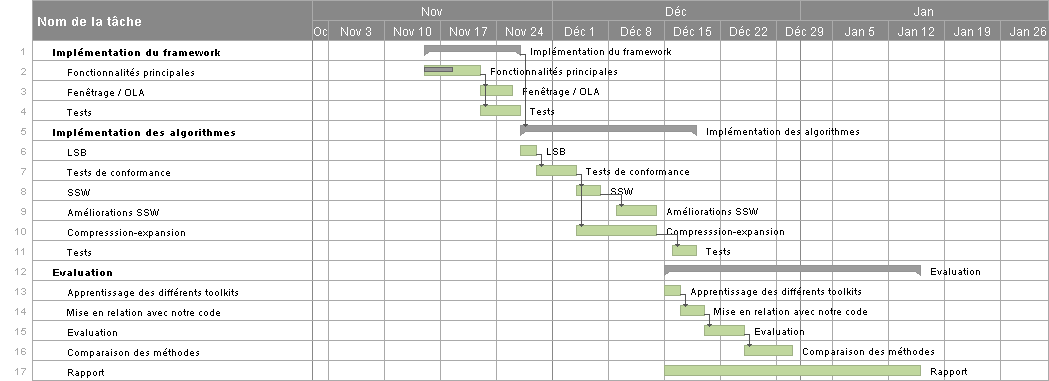
\includegraphics[scale=0.65]{images/gantt.png}
\caption{Approximative Gantt diagram for the project}
\label{gantt}
\end{sidewaysfigure}

\chapter{Implementation}
The following chapter will describe the choices and the inner workings of the project.
The implementation is divided in multiple parts (the text in fixed width font refers to the corresponding source code folder) : 

\begin{itemize}
\item An audio manipulation framework.
\item The implementation of many audio and watermarking algorithms, in this framework : the whole makes the library that we call \texttt{libwatermark}.
\item A test application to ensure correctness of the library : \texttt{lib\_testapp}.
\item A graphical interface that uses the library : \texttt{InterfaceWatermarking}.
\end{itemize}

All of these parts will be reviewed in the following sections. Theye are all thoroughly documented with \brand{Doxygen}, and the complete documentation can be found in the \texttt{doc} folder.

\section{Technologies used}
The choice was made really early to use \brand{C++} as a programming language, mostly because of the speed, but also because it is quite cross-platform. We also used many \brand{C++11} features for the sake of learning, and because it sometimes reduces the amount of code needed. However, on \brand{Microsoft Windows} with \brand{Visual Studio}, all the features might not be supported by the compiler.

\subsection{Dependencies}
We tried to use as few dependencies as possible, and we tried to choose the most cross-platform ones. In return, our software should work on every common desktop operating system, and could certainly be embedded in smartphones, etc\dots
\subsubsection{Qt}
The GUI framework. It is not used in the library, but it allowed us to make a fully working GUI in a really short amount of time; also, most of us already had some prior knowledge of it.
\subsubsection{FFTW}
This Fast Fourier Transform library has been used as the main library to perform the Fourier transform needed in some algorithms, because of its efficiency. However, other FFT libraries could be used very easily.
\subsubsection{libsndfile}
An audio file library that allows our software to open \brand{WAV} files and other common filetypes very easily. It is lightweight and efficient. Unfortunately, it doesn't support compressed formats like \brand{MP3} or \brand{OGG Vorbis}. 

\section{Framework}
An audio framework has been designed in order to streamline the audio processing operations and concentrate only on the algorithms.

The other alternatives would have been :
\begin{itemize}
\item To code every algorithm in its own function, with some helper functions to load a file, etc\dots which would have resulted in a lot less code but also a less reusable code.
\item To work in \brand{MATLAB}, which reduces the overhead needed since loading and saving files, as well as transforms, are already implemented.
\end{itemize}

A lot of effort went into making it very generic, fast, and reliable for any kind of audio operations.


\subsection{Operation}
The main idea is : 
\begin{enumerate}
\item To load some audio data.
\item To apply an algorithm to chunks (e.g. 512 samples for instance) of this data.
\item To save the result if needed.
\end{enumerate}

For instance, on a 2048 samples audio file, with a buffer size of 512, there would be four buffers that would each see the algorithm applied to them.

In the current design, there is an input and an output, input and output filters, and the algorithm. For instance, here would be the call order of a generic example.

\begin{enumerate}
\item FFT plotting \textit{calls} FFT \textit{calls} GetNextBuffer
\item Algorithm
\item IFFT \textit{calls} Waveform plotting \textit{calls} WriteNextBuffer
\end{enumerate}

However, this is somewhat clumsy to setup : one must first instantiate the original audio loader I0, then the FFT filter I1 which has to reference I0, then the plotter I2 which has to reference I1, and finally the manager class which has to reference I2, and the same for the output, which leads to bloated code and a logical dissimetry.
So in future project, the framework might be modified to take instead a list of classes which would make our example:

GetNextBuffer $\rightarrow$ FFT $\rightarrow$ FFT plotting $\rightarrow$ Algorithm $\rightarrow$ IFFT $\rightarrow$ Waveform Plotting $\rightarrow$ WriteNextBuffer.

\newpage

\subsection{Capabilities}
Since an heavy emphasis has been put into having very generic interfaces, we have been able to implement many useful features and algorithms.

The library is entirely templated, which means that most of the classes can be used with fixed or floating point numbers. However, it does not always make sense : for instance, \brand{FFTW} only works in floating point, so using \texttt{short int} as a base sample type would not work.

Multiple channels are supported in a seamless way, and can be interweaved or deinterweaved.

There are interfaces for : 
\begin{itemize}
\item Inputs and outputs \& filters.
\item Transforms.
\item Watermarking \& degradation algorithms.
\item Time management.
\item Watermark embedding.
\item Copying, overlapping and windowing.
\end{itemize}

You can see on figures \ref{frameworkclass1} to \ref{frameworkclass4} tables that repertories all the implementations of these interfaces.

\begin{figure}[h!]
\centering
\begin{tabular}{|c|c|l|}
\hline
\textbf{Inputs} & \textbf{Outputs} & \textbf{Explanation} \\
\texttt{InputManagerBase} & \texttt{InputManagerBase}  & \\
\hline
FileInput & FileOutput & Wrapper around \brand{libsndfile} \\
BufferInput & BufferOutput & Read and write from a buffer \\
SilenceInput & DummyOutput & Generates silence and writes to nothing \\
\hline
FFTInputProxy & FFTOutputProxy & FFT transform \\
MCLTInputProxy & MCLTOutputProxy & MCLT transform \\
\hline
& GnuplotOutput & Displays sample data in \brand{GNUPlot} \\
& GnuplotFFTOutput & Displays a spectrum in \brand{GNUPlot} \\
\hline
\end{tabular}

\vspace{1em}

\begin{tabular}{|c|c|l|}
\hline
\textbf{Input copy handlers} & \textbf{Output copy handlers} &  \textbf{Explanation} \\
\texttt{InputCopy} & \texttt{OutputCopy} & \\
\hline
InputSimple & OutputSimple & Copies and increment by a buffer size \\
InputOLA & OuputOLA & Copies in an overlap-add fashion \\
InputFilter & OutputFilter & Copies in order to perform convolution \\
\hline
\end{tabular}

\vspace{1em}

\begin{tabular}{|c|l|}
\hline
\textbf{Window} & \textbf{Explanation} \\
\texttt{WindowBase} & \\
\hline
RectWindow & Rectangular window : does nothing \\
BartlettWindow & Bartlett window \\
BlackmanWindow & Blackman window \\
Hann & Hann window \\
Hamming & Hamming window \\ 
\hline
\end{tabular}

\caption{Objects related to input-output}
\label{frameworkclass1}
\end{figure}

\begin{figure}[h!]
\centering
\begin{tabular}{|c|c|l|}
\hline
\textbf{Watermark encoding} & \textbf{Watermark decoding} & \textbf{Explanation} \\
\texttt{WatermarkBase} & \texttt{WatermarkBase} & \\
\hline
LSBEncode & LSBDecode & LSB algorithm \\
SSWEncode & SSWDecode & SSW algorithm \\
\hline
\end{tabular}

\vspace{1em}

\begin{tabular}{|c|l|}
\hline
\textbf{Audio degradations} & \textbf{Explanation} \\
\texttt{BenchmarkBase} & \\
\hline
AddBrumm & Adds mains-like noise \\
AddWhiteNoise & Adds white noise \\
Amplify & A simple gain \\
Convolution & Performs linear convolution for filtering (e.g. LPF / HPF)\\
Exchange & Exchanges pairs of samples \\
FFTNoise & Adds white noise using a spectral method \\
FFTAmplify & Gain using a spectral method \\
Invert & Inverts the phase of the audio \\
Smooth & Smoothes the samples \\ 
Stat1 & Also smoothes the samples \\
ZeroCross & Strict noisegate\\
\hline
\end{tabular} 
\caption{Audio algorithms}
\label{frameworkclass2}
\end{figure}

\begin{figure}[h!]
\centering
\begin{tabular}{|c|l|}
\hline
\textbf{Time management} & \textbf{Explanation} \\
\texttt{TimeAdapter} & \\
\hline
AtTime & Starts the algorithm at a certain buffer \\
Every & Starts the algorithm every $k$ buffer \\
For & Starts the algorithm for $n$ buffers \\
Every\_For & Every $k$ buffers, starts the algorithm and stops it after $n$ buffers\\
\hline
\end{tabular}
\caption{Algorithm triggering}
\label{frameworkclass3}
\end{figure}

\begin{figure}[h!]
\centering
\begin{tabular}{|c|l|}
\hline
\textbf{Watermark embedding} & \textbf{Explanation} \\
\texttt{WatermarkData} & \\
\hline
SimpleWatermarkData & Puts the watermark a single time \\   
LoopingWatermarkData & Puts the watermark repeatedly \\
\hline
\end{tabular}
\caption{Watermarked data-related objects}
\label{frameworkclass4}
\end{figure}

\newpage

\subsection{Class diagram}

The class diagram (figure \ref{classdiagram}) only shows child classes when it is relevant; else it would cause too much bloat.

Some important things to note are that :
\begin{itemize}
\item The class diagram shown here is for a generic instantiation with a watermark algorithm (it is very similar for an evaluation algorithm). 
\item Due to the complexity of the library, we will only show relevant public members and interfaces : detailed documentation is available thanks to \brand{Doxygen}.
\item Most of the classes do reference a \texttt{Parameters} class (figure \ref{parametersclass}) which holds some common parameters and types used across the library.
\item Most of the classes are templates with a \texttt{data\_type} parameter that can be \texttt{short}, \texttt{double}...
\end{itemize}


\begin{figure}[h!]
\centering
\begin{tikzpicture}
\umlclass[template=data\_type]
{Parameters}
{
	size\_type = unsigned long int \\
	complex\_type = complex<data\_type> \\
	samplingRate : size\_type \\
	bufferSize : size\_type \\	
}
{
	normFactor() : data\_type \\
}
\end{tikzpicture}

\caption{The Parameters class}
\label{parametersclass}
\end{figure}

\begin{figure}[h!]
\centering

\begin{tikzpicture}
% % % CLASS DIAGRAM HERE % % %
% Base Manager

\umlinterface[x=0,y=8]
{ManagerBase}
{}
{
	\umlvirt{prepare() : void} \\
	\umlvirt{execute() : void} \\
}

\umlclass[x=0,y=5]
{WatermarkManager}
{}
{
	\umlvirt{prepare() : void} \\
	\umlvirt{execute() : void} \\
}

% WatermarkBase
\umlinterface[x=0,y=2]{WatermarkBase}{}
{
	\umlvirt{operator()() : void} \\
}

% IO
\umlinterface[x=-6,y=6]{IOManagerBase}{}
{
	channels() : size\_type \\
	frames() : size\_type \\
	v() : vector<vector<data\_type>> \\
}
\umlinterface[x=-6,y=2]{InputManagerBase}{}
{
	getNextBuffer() : Buffer \\
}
\umlinterface[x=-5,y=-1]{OutputManagerBase}{}
{
	writeNextBuffer(Buffer) : void \\
}

% WM data
\umlinterface[x=5,y=7]{WatermarkData}{}
{
	setSize() : void\\
	nextBit() : bool\\
	setNextBit(Bool) : void \\
	isComplete() : bool \\
}

% TA
\umlinterface[x=6,y=2]{TimeAdapter}{}
{
addStartHandler(Function) : void\\
addStopHandler(Function) : void\\
perform() : void \\
}
% Links
\umlinherit{WatermarkManager}{ManagerBase}
\umlinherit{InputManagerBase}{IOManagerBase}
\umlinherit{OutputManagerBase}{IOManagerBase}

\umlaggreg{InputManagerBase}{WatermarkManager}
\umlaggreg{OutputManagerBase}{WatermarkManager}
\umlaggreg{WatermarkBase}{WatermarkManager}
\umlaggreg{WatermarkData}{WatermarkManager}
\umlaggreg{TimeAdapter}{WatermarkManager}

\end{tikzpicture}

\caption{Class diagram for the main usage of the framework}
\label{classdiagram}
\end{figure}

\newpage

\subsection{Example of usage}
We will here have a look at an example usage of our library which will correspond to the encoding of some bits with the LSB algorithm.

More examples can be seen in the test application.

\begin{figure}[h!]
\centering

\begin{lstlisting}
    Parameters<short> conf;
    
    WatermarkData* data = new SimpleWatermarkData; // Set the bits afterwards 
    auto input = new FileInput<short>("input_mono.wav", conf);
    auto output = new FileOutput<short>(conf);

    auto algorithm = new LSBEncode<short>(conf);

    WatermarkManager manager(Input_p(input),
    						 Output_p(output),
    						 Watermark_p(new LSBEncode<short>(conf)),
    						 WatermarkData_p(data));
    manager.execute();

    output->writeFile("lsb_encode.wav");
\end{lstlisting}

\caption{Example instanciation}
\end{figure}

\newpage

\section{Algorithms}
\subsection{Watermarking and evaluation algorithms}
They are separated in two folders : \texttt{benchmark} and \texttt{watermark}.

We tried very hard to use the \brand{C++11} features efficiently in our code.

Here is for instance the code that performs the \texttt{Amplify} operation : 

\begin{figure}[ht!]
\centering
\begin{lstlisting}
			for(auto& sampleData : channelsData)
			{
				MathUtil::apply(sampleData,
				[&] (data_type x)
				{
					return x * _gain;
				});
			}
\end{lstlisting}
\caption{Amplify algorithm}
\label{amplify}
\end{figure}

It reads very easily : "For each channel, multiply the whole channel by the gain", thanks to lamda-expressions and range-based for-loop.

We also made our system so that the user of our framework can choose when does the effect starts, how long it should last, and if it repeats. The granularity is the buffer size.

For instance, in order to make some benchmarks, it is possible to make a volume modification using the algorithm on fig. \ref{amplify} every 80 buffers, for 5 buffers, starting at 200 buffers.
\subsection{Transforms}
The main problem with transforms is that they might be transforming from and to different domains.
Hence, instead of forcing the use of an interface directly on the object making the transform, which would cause awkward inheritance and overloading problems, we force the interface on the input and output proxies : they have to follow the interface of \texttt{InputManagerBase} and \texttt{OutputManagerBase}.

\subsubsection{Fourier transform}
The Fourier transform uses \brand{FFTW} but can easily be adapted to use any other library or custom code.
The functions used are \texttt{fftw\_plan\_dft\_r2c\_1d} and \texttt{fftw\_plan\_dft\_c2r\_1d} : hence the resulting output array 
only holds the $\frac{N}{2} + 1$ relevant coefficients ($N$ being the number of input samples), and not the symmetrical ones.

\subsubsection{Modulated complex lapped transform}
This transform was referred to in \cite{malvar1999modulated}. It seems that it can provide better results with the spread-spectrum technique. However our implementation assumes that the Fourier transform has already been applied to the buffer.

\section{Tests}
The tests referred here are only there to check that the algorithms are properly implemented and that for instance a watermark can be retrieved without problems..

Every object is tested and produces an audio file which is then either manually (for benchmarks for instance) or automatically (for watermark embedding and reading) checked. The \brand{QtTest} framework is used.

The testing of core features (e.g. transforms, overlap, windowing, etc...) is achieved by null-testing to the reference audio and checking that the RMS value of the difference is not too high.
\section{GUI}
\subsection{Capabilities}
Here is a non-exhaustive list of the capabilities of our graphical interface.
\begin{itemize}
\item Loading and saving audio files.
\item Watermark inputting, embedding and reading.
\item Waveform display.
\item Application of degradations.
\item Display of the capacity available in the file in real time.
\item Multiple configuration options, that can be saved and loaded.
\end{itemize}
\subsection{Screenshots}
\section{Evaluation}
\chapter{Results}
\label{chap:results}
\section{Evaluation results}
The evaluation has been made for the \ac{LSB} (the reference), the \ac{RLSB} and the \ac{SSW} technique with the \texttt{Amplify}, \texttt{Convolution} (with a low-pass filter) and \texttt{FFTAmplify} degradations. The scores (number of false bits) are :

\begin{figure}[h!]
\centering
\begin{tabular}{|c|c|c|c|}
\hline
\backslashbox{Algorithm}{Degradation} & \texttt{Amplify} & \texttt{Convolution} & \texttt{FFTAmplify} \\
\hline
\ac{LSB} & 5 & 10 & 7 \\
\hline
\ac{RLSB} & 31 & 37 & 7\\
\hline
\ac{SSW} & 52 & 71 & 52\\
\hline
\end{tabular}
\end{figure}
\section{Auditory results}
The auditory evaluation, made on about ten persons, wasn't really relevant. The watermark made on the audio files were audible, all of the persons reported a difference. Added to this, the audio files watermarked with the LSB method showed lot of noise, the original song wasn't audible. The experiment with the SSW technique were more relevant as the song was still audible.
\chapter*{Conclusion}

\bibliographystyle{plainnat}
\bibliography{watermarking}
\end{document}
